\documentclass{beamer}
\mode<presentation> {
%\usetheme{Dresden}
\usetheme{CambridgeUS}
}
\newcommand{\subitem}{\par\qquad}
\usepackage{booktabs}
\usepackage{algorithm}
\usepackage{algorithmic}
\usepackage{tikz}
\usepackage{subfigure}	
\usepackage[round]{natbib}   % omit 'round' option if you prefer square brackets
\DeclareMathOperator*{\argmin}{argmin}
\DeclareMathOperator*{\argmax}{argmax}

\usetikzlibrary{arrows,calc,positioning,decorations.pathreplacing} 
\tikzset{
	>=stealth',
	punkt/.style={
		circle,
		draw=black, thick,
		minimum height=2em,
		inner sep=0pt,
		text centered},
	pil/.style={
		->,
		thick,
		shorten <=2pt,
		shorten >=2pt,},
	cir/.style={
		rectangle,
		rounded corners,
		draw=black, thick,
		minimum width=1.5em,
		text centered},
	arr/.style={
		->,
		thick,
		shorten <=2pt,
		shorten >=2pt,},
	layer/.style={
		draw=black,
		fill=white,
		thick,
		rectangle,
		rounded corners,
		minimum width=1.5em,
		minimum height=12em
	},
	brace/.style={
		thick,
		decoration={
			brace,
			mirror,
			raise=2.5cm
		},
		decorate
	}
}

\newcommand{\drawlayer}[4]{
	\node[layer, draw=#4] (#1) at (#2,#3) {};
	\foreach \x in {-1.75, -1.25, -0.75, -0.25, 0.25, 0.75, 1.25, 1.75} \draw[thick, #4] (#2,\x+#3) circle (0.15);
}
\newcommand\irregularcircle[2]{
	\pgfextra {\pgfmathsetmacro\len{(#1)+rand*(#2)}}
	+(0:\len pt)
	\foreach \a in {10,20,...,350}{
		\pgfextra {\pgfmathsetmacro\len{(#1)+rand*(#2)}}
		-- +(\a:\len pt)
	} -- cycle
}

\newcommand{\independent}{\mbox{${}\perp\mkern-11mu\perp{}$}}
\newcommand{\notindependent}{\mbox{${}\not\!\perp\mkern-11mu\perp{}$}}
\newcommand{\iid}{\overset{\text{iid}}{\sim}}

%%%%%%%%%%%%%%%%%%%%%%%%%%%%%%%%%%%%%%%%%%%%%%%%%%%%%%%%%%%%%%%%%%%%%%%%%%
% PARENTHESES 
%%%%%%%%%%%%%%%%%%%%%%%%%%%%%%%%%%%%%%%%%%%%%%%%%%%%%%%%%%%%%%%%%%%%%%%%%%

\renewcommand{\dot}[2]{\langle {#1},\, {#2} \rangle}
\newcommand{\pa}[1]{\left( #1 \right)}
\newcommand{\pb}[1]{\left\{ #1 \right\}}
\newcommand{\pc}[1]{\left[ #1 \right]}
\newcommand{\pn}[1]{\left\| #1 \right\|}
\newcommand{\ps}[1]{\left| #1 \right|}
\newcommand{\ot}{\leftarrow}
\newcommand{\given}{\, | \,}

%%%%%%%%%%%%%%%%%%%%%%%%%%%%%%%%%%%%%%%%%%%%%%%%%%%%%%%%%%%%%%%%%%%%%%%%%%
% MATHCAL
%%%%%%%%%%%%%%%%%%%%%%%%%%%%%%%%%%%%%%%%%%%%%%%%%%%%%%%%%%%%%%%%%%%%%%%%%%

\newcommand{\D}{\mathcal{D}}
\renewcommand{\P}{\mathcal{P}}
\renewcommand{\Pr}{\mathbb{P}}
\renewcommand{\H}{\mathcal{H}}
\renewcommand{\L}{\mathcal{L}}
\newcommand{\Hk}{{\mathcal{H}_k}}
\newcommand{\F}{\mathcal{F}}
\newcommand{\X}{\mathcal{X}}
\newcommand{\Y}{\mathcal{Y}}
\newcommand{\Z}{\mathcal{Z}}
\newcommand{\N}{\mathcal{N}}
\newcommand{\Ex}{\mathcal{E}}
\newcommand{\Hyp}{\mathcal{H}}
\newcommand{\B}{\mathcal{B}}


%%%%%%%%%%%%%%%%%%%%%%%%%%%%%%%%%%%%%%%%%%%%%%%%%%%%%%%%%%%%%%%%%%%%%%%%%%
% MATHBB 
%%%%%%%%%%%%%%%%%%%%%%%%%%%%%%%%%%%%%%%%%%%%%%%%%%%%%%%%%%%%%%%%%%%%%%%%%%

\newcommand{\Pio}{\mathbb{P}}
\newcommand{\R}{\mathbb{R}}
\newcommand{\Rd}{\mathbb{R}^d}
\newcommand{\Rq}{\mathbb{R}^q}
\newcommand{\Rn}{\mathbb{R}^n}
\newcommand{\Rm}{\mathbb{R}^m}
\newcommand{\Rnd}{\mathbb{R}^{n \times d}}
\newcommand{\Rnm}{\mathbb{R}^{n \times m}}
\newcommand{\I}{\mathbb{I}}
\newcommand{\Pa}{\mathrm{Pa}}
\renewcommand{\d}{\mathrm{d}}
\newcommand{\sig}{\mathrm{sign}\circ\!}
\newcommand{\Rp}{R_{\varphi}}
\newcommand{\Rpn}{\hat{R}_{\varphi}}
\newcommand{\Rpnt}{\tilde{R}_{\varphi}}
\newcommand{\f}{f^*}
\newcommand{\fn}{\hat{f}_n}
\newcommand{\fnt}{\tilde{f}_n}
\newcommand{\fntm}{\tilde{f}^m_n}
\newcommand{\Mk}{\M_k}
\newcommand{\muP}{\mu_k(\P)}
\renewcommand{\d}{{\mathrm{d}}}
\newcommand{\Rad}{\mathrm{Rad}}
\newcommand{\M}{\mathscr{M}}
\newcommand{\head}[2]{\multicolumn{1}{>{\centering\arraybackslash}p{#1}}{\textbf{#2}}}
\renewcommand{\do}{do}
\title[Likelihood-Free Overcomplete ICA]{Likelihood-Free Overcomplete ICA and Applications in Causal Discovery} 

\author[Behrad Moniri]{Behrad Moniri}

\institute[Causal AI - EE @ Sharif] 
{
Department of Electrical Engineering\\
Sharif University of Technology 
}

\titlegraphic{
\includegraphics[width=2cm]{logo.png}\hspace*{-8.75cm}~%
%	\includegraphics[width=2cm]{digilogo.png}
}
\newcommand{\bigCI}{\mathrel{\text{\scalebox{1.07}{$\perp\mkern-10mu\perp$}}}}

\begin{document}

\begin{frame}
\titlepage
\end{frame}

\begin{frame}
\frametitle{General Framework}
Linear ICA assumes the following data generation model:
\begin{equation}
\label{equ:ica}
\mathbf{x} = \mathbf{As},
\end{equation}
where $\mathbf{x}\in \mathbb{R}^{p}, \mathbf{s}\in \mathbb{R}^{d}, \mathbf{A}\in \mathbb{R}^{p\times d}$

\begin{itemize}
\item
The elements in $\mathbf{s}$ are supposed to be independent from each other.
\item
each follows a non-Gaussian distribution (or at most one of them is Gaussian).
\item
The goal of ICA is to recover both $\mathbf{A}$ and $\mathbf{s}$ from observed mixtures $\mathbf{x}$.

\item
In causal discovery, the main goal is to recover a constrained $\mathbf{A}$ matrix. When $d>p$, the problem is known as overcomplete ICA (OICA).
 \end{itemize}
\end{frame}

\begin{frame}
\frametitle{Liklihood-Based Methods of Source Separation}

Whenever there are hidden confounders, causal discovery and with the linearity and non-Gaussian noise constraints,  the corresponding causal discovery algorithms can be seen as extension of overcomplete independent componentanalysis (OICA). 


Unlike regular ICA, in which the mixing matrix is invertible, OICA is not!

\end{frame}

\begin{frame}
\begin{itemize}
\item
Exisiting OICA algorithms typically assume a parametric distribution for the ICs.
\item
For example, if assuming each IC follows a Mixture of Gaussian(MoG)  distribution,  one  can  simply  derive  the  likelihood  for  the  observed  data.
\end{itemize}
\end{frame}


\begin{frame}
\begin{equation}
\label{equ:generatemixtures}
\hat{\mathbf{x}} = \mathbf{A}[\hat{s}_1,\ldots,\hat{s}_d]^\intercal=\mathbf{A}[f_{\theta_1}(z_1),\ldots,f_{\theta_d}(z_d)]^\intercal=G_{\mathbf{A}, \boldsymbol{\theta}}(\mathbf{z}),
\end{equation}
where $\boldsymbol{\theta}=[\theta_1,\ldots,\theta_d]^\intercal$ and $\mathbf{z}=[z_1,\ldots,z_d]^\intercal$.

\begin{figure}[h]
	\frametitle{Paper's Contribution}
	\centering
	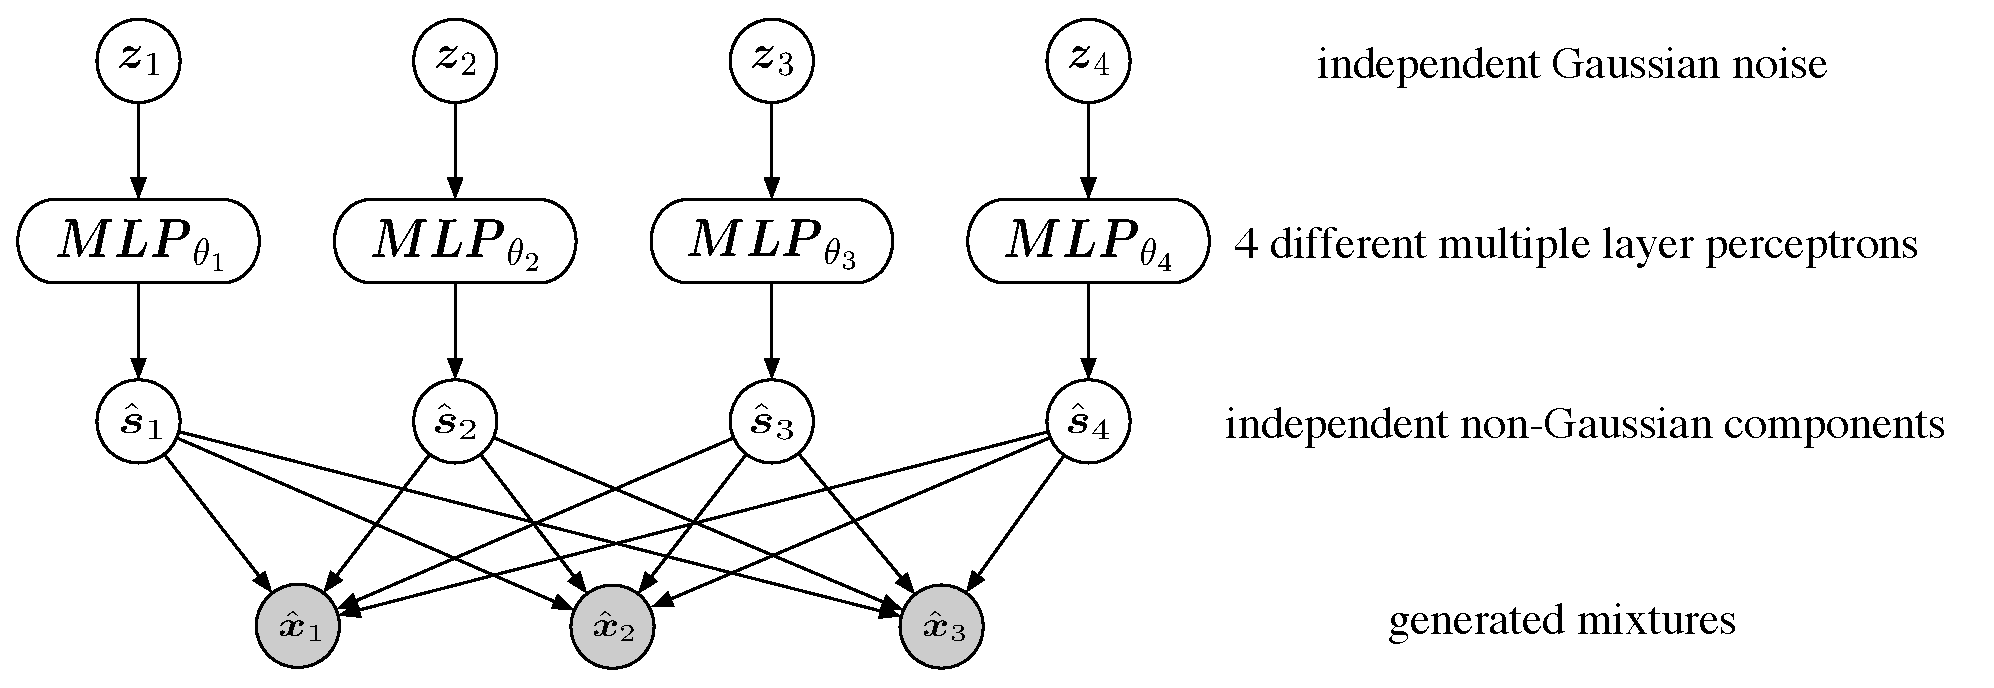
\includegraphics[width=0.8\textwidth]{overcomplete_ica.eps}
	\caption{generator architecture of LFOICA. ${z}_1, {z}_2, {z}_3, {z}_4$ are i.i.d Gaussian noise variables.}
	\label{fig:overcompleteica}
\end{figure}
\end{frame}

\begin{frame}
While most of the previous algorithms for both undercomplete  and overcomplete scenarios try to minimized the dependence among the recovered components, the components $\hat{s}_i$ recovered by LFOICA are essentially independent because the noises ${z}_i$ are independent, according to the generating process.
\end{frame}

\begin{frame}
The LFOICA generator $G_{\mathbf{A}, \boldsymbol{\theta}}$ can be learned by minimizing the distributional distance between the data sampled from the generator and the observed $\mathbf{x}$ data. 
\begin{flalign}
\label{equ:opt}
\mathbf{A}^*, \boldsymbol{\theta}^*&=\argmin \limits_{\mathbf{A}, \boldsymbol{\theta}}M\left(\mathbb{P}(\mathbf{x}\right), \mathbb{P}(G_{\mathbf{A}, \boldsymbol{\theta}}(\mathbf{z})))\nonumber\\
&=\argmin \limits_{\mathbf{A}, \boldsymbol{\theta}}\left\|\mathbb{E}_{\mathbf{x}\sim p(\mathbf{x})} [\phi\left(\mathbf{x}\right)]-\mathbb{E}_{\mathbf{z}\sim p(\mathbf{z})} [\phi\left(G_{\mathbf{A}, \boldsymbol{\theta}}(\mathbf{z})\right)]\right\|^{2},
\end{flalign}

In practice, we optimize some empirical estimator of (\ref{equ:opt}) on minibatches by stochastic gradient descent (SGD).
\end{frame}


\begin{frame}
\begin{figure}
	
\includegraphics[scale=0.3]{alg.png}
\end{figure}

\end{frame}

\begin{frame}
\frametitle{Identifiability Results}
\begin{theorem}
Given two OICA models $\textbf{x}=G_{\mathbf{A}, \theta}(\textbf{x})$ and $\textbf{x'} = G_{\mathbf{A'}, \theta'}(\textbf{z'})$ that specify distributions $\mathbb{P}(\textbf{x})$ and $\mathbb{P}(\textbf{x'})$, respectively.  Under the non-Gaussian assumption off $f(z_i)$, if $MMD(\mathbb{P}(\textbf{x'}),\mathbb{P}(\textbf{x})) = 0$, then $A'=AP_pS_p$, where Pp is a $p\times p$ column permutation matrix and $S_p$ is a $p\times p$ scaling matrix.
\end{theorem}
\begin{itemize}
\item
Cites an old ICA paper (in TSP) for proof! This theorem was only added in the final version of paper.\\
\pause
\item
$\theta$ is NOT identifiable!
\end{itemize}
\end{frame}

\begin{frame}
\frametitle{Practical Consideration}
\begin{itemize}
\item
Mixing matrix is sparse in many real systems, we add a LASSO regularizer to (\ref{equ:opt}), resulting in the loss function $M\left(\mathbb{P}(\mathbf{x}\right), \mathbb{P}(G_{\mathbf{A}, \boldsymbol{\theta}}(\mathbf{z})))+\lambda \sum_i\sum_j|\mathbf{A}_{ij}|$.

\item 
Typical proximal methods can be used to solve this problem.
\end{itemize}
\end{frame}


\begin{frame}
\frametitle{Causal Discovery under Measurement Error}
\begin{itemize}
\item
LiNGAM model for variables without measurement error:
$\textbf{X} = \mathbf{B}\mathbf{\tilde{X}} + \mathbf{\tilde{E}}$
\item Measurement error:
$\textbf{X} = \mathbf{\tilde{X}} + \textbf{E}$

\begin{align}
\label{equ:measurementerror}
\mathbf{X} = \tilde{\mathbf{X}} + \mathbf{E}&=(\mathbf{I}-\mathbf{B})^{-1} \tilde{\mathbf{E}} +\mathbf{E}
=\left[(\mathbf{I}-\mathbf{B})^{-1}\quad \mathbf{I}\right]\left[\begin{array}{c}
\tilde{\mathbf{E}}\\
\mathbf{E}
\end{array}\right]
\end{align}

\item Fits well within the OICA framework.
\end{itemize}
\end{frame}

\begin{frame}
\frametitle{Subsampled Time Series}
\begin{itemize}
	\item Original "Causal Frequency" follow VAR(1):	
\begin{equation}
\label{equ:originalprocess}
\mathbf{x}_t=\mathbf{A}\mathbf{x}_{t-1}+\mathbf{e}_t,
\end{equation}

\item Sum-sampling with factor $k$:
\begin{align} 
\label{equ:subsample}
\tilde{\mathbf{x}}_{t+1}=\mathbf{A}^k\mathbf{\tilde{x}}_t+\mathbf{L\tilde{e}}_{t+1}
\end{align}
Where $\tilde{\mathbf{x}}$ is the observed data subsampled from $\mathbf{x}$, $\mathbf{L}= [\mathbf{I, A, A^2, ..., A^{k-1}}], \mathbf{\tilde{e}} = (\mathbf{e}_{1+tk-0}^\intercal, \mathbf{e}_{1+tk-1}^\intercal, ..., \mathbf{e}_{1+tk-(k-1)}^\intercal)^\intercal \notag$.  We are interested in estimating the transition matrix $\mathbf{A}$ from the subsampled data.
\end{itemize}
\end{frame}

\begin{frame}
\frametitle{Idea! Conditional GAN}
\begin{align} 
\label{equ:subsample}
\tilde{\mathbf{x}}_{t+1}=\mathbf{A}^k\mathbf{\tilde{x}}_t+\mathbf{L\tilde{e}}_{t+1}
\end{align}
\begin{figure}
	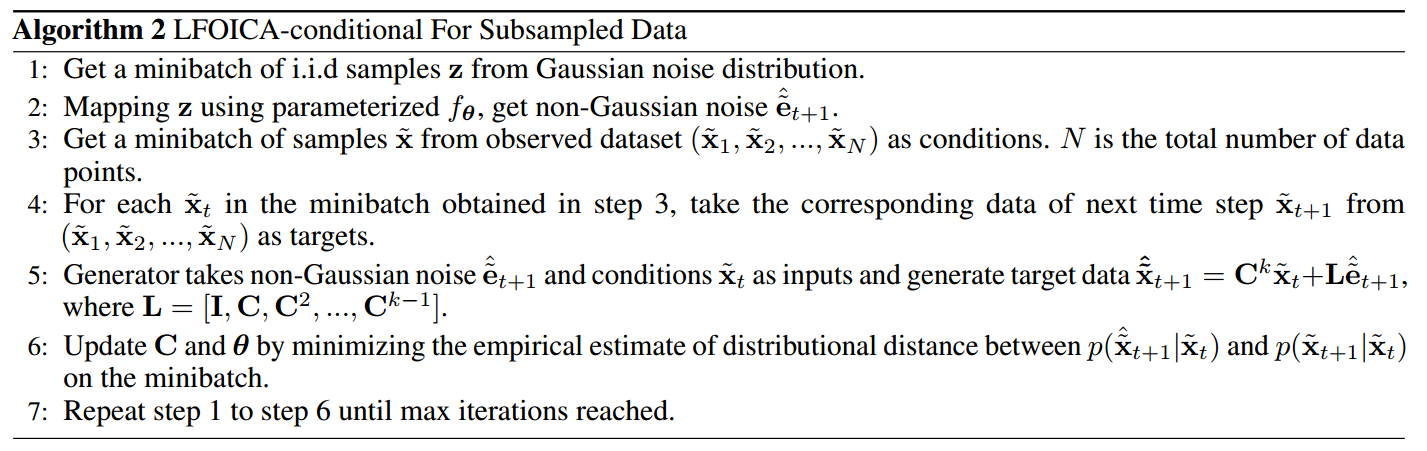
\includegraphics[scale=0.23]{algg.png}
\end{figure}
\begin{figure}
	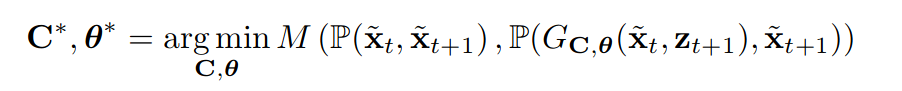
\includegraphics[scale=0.3]{MIn.png}
\end{figure}
\end{frame}

\begin{frame}
\begin{figure}
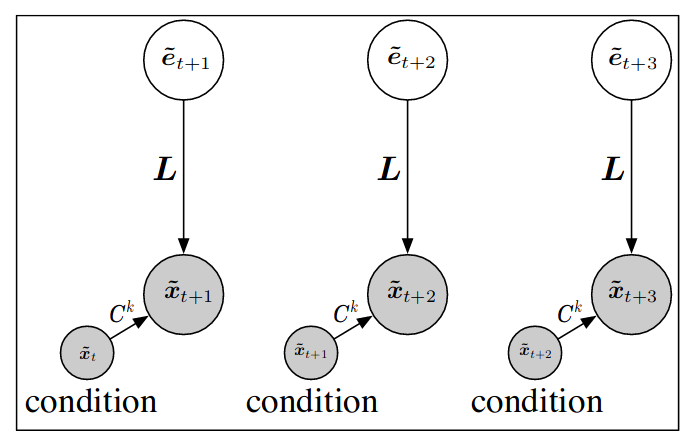
\includegraphics[scale=0.3]{cond.png}
\end{figure}
\end{frame}
\end{document}

